\documentclass[onecolumn,3p]{elsarticle}
\makeatletter
\def\ps@pprintTitle{%
	\def\@oddfoot{}%
	\let\@evenfoot\@oddfoot}
\makeatother
\usepackage{latexsym,amssymb,amsmath}
\usepackage[tiny]{titlesec}
\usepackage{graphicx}
\usepackage{float}
\usepackage{enumitem}
\usepackage{hyperref}

\begin{document}
	\begin{frontmatter}
		\title{Trajectory-free calculation of attracting and repelling manifolds}
		\author{Gary K. Nave Jr.}
		\ead{gknave@vt.edu}
		
		\author{Shane D. Ross}
		
		\address{Engineering Mechanics Program, Virginia Tech}
		
		\begin{abstract}
			We develop a method for finding attracting or repelling hyperbolic Constrained Eulerian Coherent Structures (CECSs) in autonomous 2-dimensional systems. We take a small time approximation of the trajectory-normal repulsion factor and find its leading-order behavior, which represents the infinitesimal stretching of normal vectors to trajectories throughout the flow. The resulting repulsion rate does not require the computation of trajectories and therefore independent of any calculation parameters such as integration time. We show its application to several systems, including slow-fast system for discovery of their slow manifolds.
		\end{abstract}
	\begin{keyword}
		Coherent Structures \sep Invariant manifolds \sep Slow-fast systems
	\end{keyword}
	\end{frontmatter}

	\section{Introduction}
	Over the past few decades, a variety off computational techniques have been introduced to understand the underlying behaviors of dynamical systems based on the geometric structures within their flow. These coherent structures have been applied to better understand plant pathogen spread \cite{schmale2015highways}, seabird foraging trips \cite{kai2009top}, planetary motion \cite{gawlik2009lagrangian}, and ocean flows \cite{wiggins2005dynamical}. By detecting and analyzing the underlying structures of flows, we gain a better understanding of the system.
	
	There are many Lagrangian methods for detecting coherent structures, most of which use numerical integration of trajectories to characterize the flow. A fantastic comparison between these Lagrangian methods can be found in the recent work of Hadjighasem et al. \cite{hadjighasem2017critical}. These trajectory calculations may be very computationally expensive, causing a very large calculation time for computational Lagrangian methods. Therefore, it would be advantageous to develop methods which can detect coherent structures through information about the instantaneous flow map itself. In the present work, we introduce a trajectory-free method for calculating coherent structures based on the short-time behavior of the system.
	
	%The identification of geometric structures lies at the heart of the study of dynamical systems, dating all the way back to the identification of equilibria and the analysis of their stability. For autonomous systems, equilibrium points are $0$-dimensional invariant manifolds that govern the flow around them. In many systems, there are higher-dimensional structures which provide additional structure to the flow. These structures provide the skeleton of the flow, while equilibria provide the joints. These coherent structures provide understanding and intuition about the system's behavior.
	
	%If we constrain our search for coherent structures to the invariant manifolds within the flow, which, for an autonomous system are simply the trajectories, it simplifies our search for coherent structures. Researchers have developed techniques for finding these constrained Lagrangian coherent structures

	\section{Background}
	To begin, consider a general two-dimensional autonomous ordinary differential equation
	\begin{equation}
		\mathbf{\dot x} = \mathbf{v}(\mathbf{x}), \quad \mathbf{x} \in U \subseteq \mathbb{R}^2
	\end{equation}
	with its one-parameter flow map,
	\begin{equation}
		\begin{split}
			& \mathbf{F}^T : U \rightarrow U, \quad T \in \mathbb{R} \\
			& \mathbf{x}_0 \mapsto \mathbf{x}_T = \mathbf{x}(T,0,\mathbf{x}_0)
		\end{split}
	\end{equation}
	For any $\mathbf{x} \in U$ with $\mathbf{v}(\mathbf{x}) \ne \mathbf{0}$ (i.e., excluding equilibrium points), we define the following unit vector fields parallel and normal to the governing vector field $\mathbf{v}(\mathbf{x})$, respectively,
	\begin{equation}
		\begin{split}
			& \mathbf{e}(\mathbf{x}) = \frac{\mathbf{v}(\mathbf{x})}{|\mathbf{v}(\mathbf{x})|}, \\
			& \mathbf{n}(\mathbf{x}) = \mathbf{R} \mathbf{e}(\mathbf{x})
			, \quad   
			\mathbf{R} = \left(
			\begin{array}{cc}
			0 & -1 \\
			1 & ~ 0 
			\end{array}
			\right)
		\end{split}
		\label{unit_vector_fields}
	\end{equation}
	
	\subsection{Trajectory-normal repulsion factor}
	For any trajectory passing through a point $\mathbf{x}_0 \in U$ with 
	$\mathbf{v}(\mathbf{x}_0) \ne \mathbf{0}$, we define locally the {\it trajectory-normal repulsion factor}\footnote{Note that Haller \cite{haller_variational_2011} used the name `repulsion rate', but we believe the term `rate' should be reserved for another quantity.} $\rho_T(\mathbf{x}_0)$ over the time interval $[0, T]$ as  the projection of $\nabla\mathbf{F}^T (\mathbf{x}_0) \mathbf{n}_0 $ onto the new normal 
	$\mathbf{n}_T$,
	\begin{equation}
		\rho_T(\mathbf{x}_0) = \langle  \mathbf{n}_T , \nabla \mathbf{F}^T (\mathbf{x}_0) \mathbf{n}_0 \rangle
	\end{equation}
	where $\mathbf{n}_T = \mathbf{n}(\mathbf{x}_T) = \mathbf{n}(\mathbf{F}^T (\mathbf{x}_0))$. 
	As illustrated in Figure \ref{fig:normal-repulsion-factor-2D}, $\rho_T(\mathbf{x}_0)$ is a measure of the growth of infinitesimal perturbations normal to the invariant manifold $\mathcal{M}$ containing $\mathbf{x}_0$ over the time interval $[0,T]$.
	If the projection $\rho_T(\mathbf{x}_0) >1$, we have growth of infinitesimal perturbations normal to the trajectory through $\mathbf{x}_0$ over the time interval $[0,T]$.
	\begin{figure}[t]
		\centering
		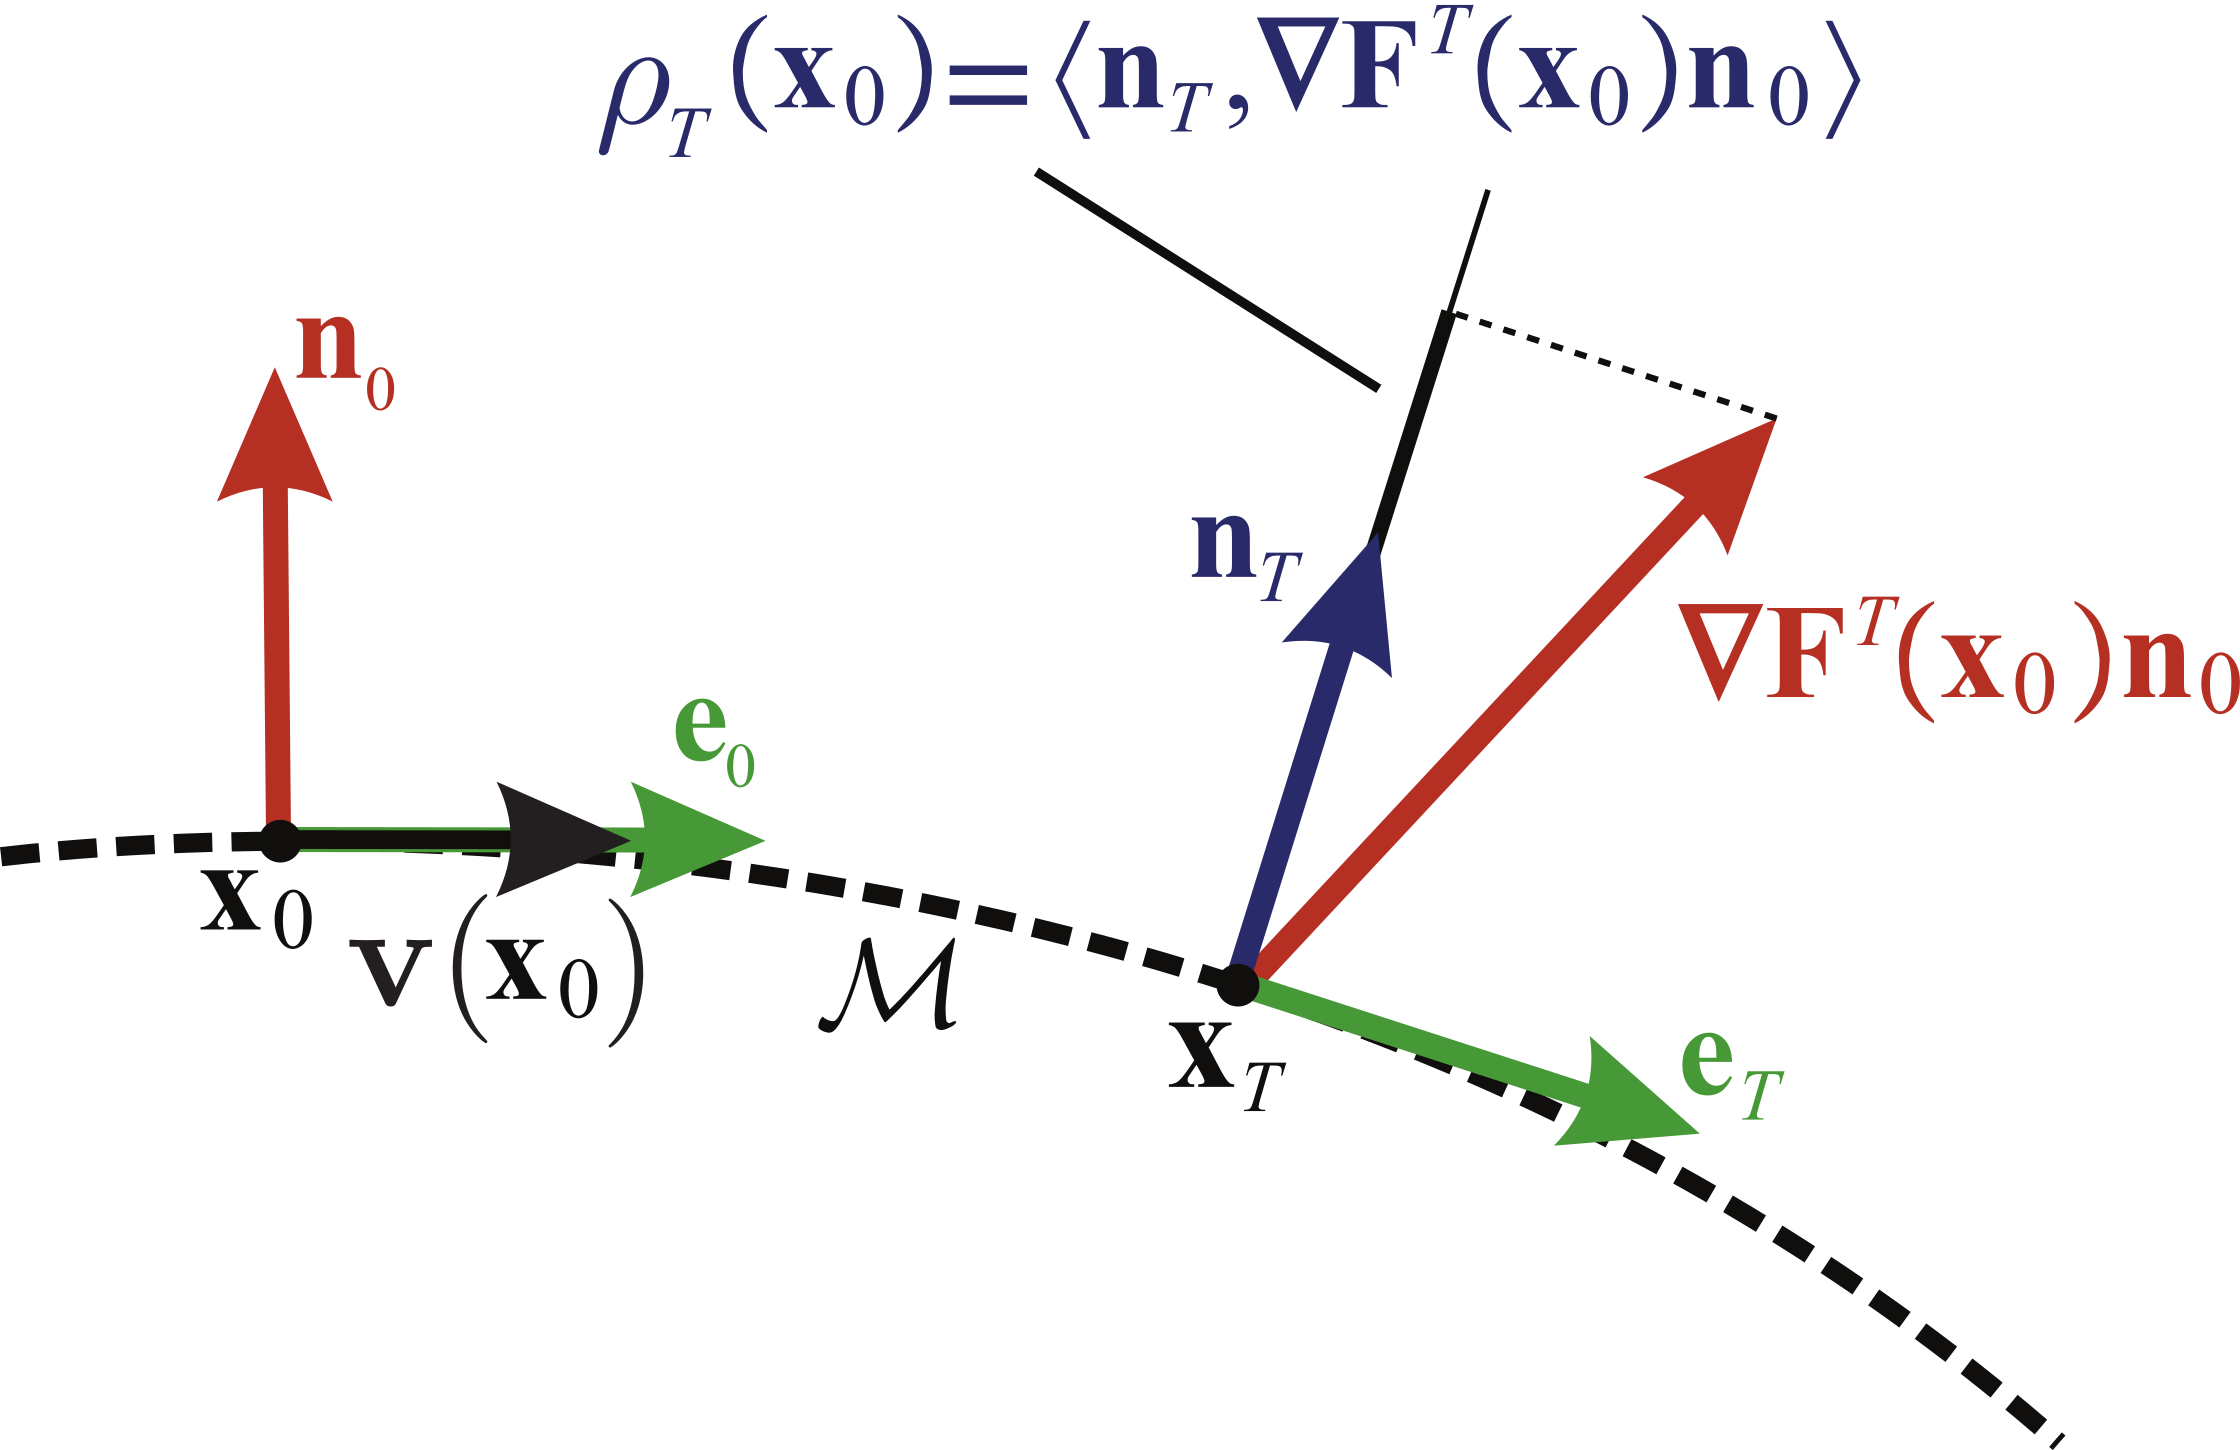
\includegraphics[width=0.45\textwidth]{normal-repulsion-factor-2D.png}
		\caption{Geometry of the trajectory-normal repulsion factor, modified from \cite{haller_variational_2011}.}
		\label{fig:normal-repulsion-factor-2D}
	\end{figure}
	
	The scalar field $\rho_T(\mathbf{x}_0)$  can be used to extract the most influential invariant manifolds, in the sense that it reveals those manifolds that normally repel (or attract) other manifolds at the largest rate. Using this trajectory-normal repulsion factor, we can discover, for example, {\it slow-manifolds}, such as those found in the following examples below.
	
	\subsection{Trajectory-normal repulsion ratio}
	A related quantity is the {\it trajectory-normal repulsion ratio}, which is the ratio of repulsion in the normal direction to the tangential stretching along a trajectory passing through the point $\textbf{x}_0$ over the time interval $[0, T]$.
	\begin{equation}
		\nu_T(\mathbf{x}_0) = \frac{\rho_T(\mathbf{x}_0)}{\left|\nabla\mathbf{F}^T (\mathbf{x}_0) \mathbf{e}_0\right|}
	\end{equation}
	
	Where the trajectory-normal repulsion ratio \(\nu_T(\mathbf{x}_0)>1\), the normal stretching dominates the tangential stretching of the curve.
	
	\subsection{Constrained Lagrangian coherent structures}
	Using both these scalar fields, Haller \cite{haller_variational_2011} formalizes the conditions for {\it constrained Lagrangian coherent structures} (CLCS). CLCSs are ridges in the $\rho_T$-field that represent the most attracting or repelling invariant manifolds in the flow of a dynamical system. For a two-dimensional autonomous system, each trajectory is an invariant manifold. Therefore, the CLCS in an autonomous system are the trajectories which are the most attracting or repelling. \\
	
	\noindent \textbf{Conditions for constrained LCS (from \cite{haller_variational_2011}, Theorem 20).} An invariant manifold $\mathcal{M}$ is a {\it weak} constrained Lagrangian coherent structure if and only if
	\begin{enumerate}[label=1\alph*.]
		\item $\rho_T(\mathbf{x}_0) > 1$
		\item $\nu_T(\mathbf{x}_0) > 1$
		\item $\langle \nabla \rho_T(\mathbf{x}_0), \mathbf{n}(\mathbf{x}_0) \rangle = 0 \quad \forall \, \mathbf{x}_0 \in \mathcal{M}$
	\end{enumerate}
		
	An invariant manifold $\mathcal{M}$ is a constrained Lagrangian coherent structure if and only if
	\begin{enumerate}[label=2\alph*.]
		\item $\mathcal{M}$ to is a weak CLCS.
		\item $\langle \mathbf{n}(\mathbf{x}_0), \nabla^2\rho_T(\mathbf{x}_0)\mathbf{n}(\mathbf{x}_0) \rangle < 0 \quad \forall \, \mathbf{x}_0 \in \mathcal{M}$ \\
	\end{enumerate}
	
	Note that both the trajectory-normal repulsion factor and trajectory-normal repulsion ratio can be written in terms of the right Cauchy-Green tensor $\mathbf{C}^T (\mathbf{x}_0)$, well-known from its use in FTLE and LCS calculations, as in \cite{haller_variational_2011},
	\begin{equation}
		\begin{aligned}
		\rho_T(\mathbf{x}_0) 
		& = \sqrt{ \frac{
				\left| \mathbf{v}(\mathbf{x}_0)\right|^2 {\rm det} \mathbf{C}^T (\mathbf{x}_0)}{
				\langle \mathbf{v}(\mathbf{x}_0),\mathbf{C}^T (\mathbf{x}_0) \mathbf{v}(\mathbf{x}_0) \rangle
			} } \\
		\nu_T(\mathbf{x}_0) 
		& =  \frac{
				\left| \mathbf{v}(\mathbf{x}_0)\right|^2 \sqrt{{\rm det} \mathbf{C}^T (\mathbf{x}_0)}}{
				\langle \mathbf{v}(\mathbf{x}_0),\mathbf{C}^T (\mathbf{x}_0) \mathbf{v}(\mathbf{x}_0) \rangle
			}
		\end{aligned}
		\label{eq: rhoT}
	\end{equation}
	As a matter of notation, in this work, we will use \((\cdot)^T\) or \((\cdot)_T\) to indicate a value over the interval $[0, T]$ and \((\cdot)^*\) to indicate the matrix transpose. Note that $T$ can be positive or negative. 
	
	We will also consider the instantaneous limit $T \rightarrow 0$ for $\rho_T(\mathbf{x}_0)$ which yields $\dot \rho(\mathbf{x}_0)$, the scalar field of the  {\it trajectory-normal repulsion rate}, for which we do not even need to calculate trajectories.
	
	\section{Constrained Eulerian coherent structures}
	The trajectory-normal repulsion factor, \(\rho_T\) can be useful in finding attracting (or repelling) structures in a flow. For scalar and tensor fields, we will drop the dependence on $\mathbf{x}_0$ for clarity.
	For small time \(T\), \cite{serra_objective_2016} introduce the following expansion for \(\mathbf{C}^T  \)
	\begin{equation}
	\mathbf{C}^T   = \mathbf{I} + 2 T \mathbf{S}  
	+ \mathcal{O}(T^2)
	\label{eq: CG Expansion}
	\end{equation}
	where $\mathbf{S}  $ is the symmetric (Eulerian) rate-of-strain tensor,
	\begin{equation}
	\mathbf{S}   = \tfrac{1}{2} \left( \nabla \mathbf{v}  + \nabla \mathbf{v} ^* \right)
	\end{equation}
	For $n=2$ dimensions,
	\begin{equation}
	{\rm det} (\mathbf{A} + \mathbf{B}) = {\rm det} \mathbf{A} + {\rm det} \mathbf{B} + {\rm det} \mathbf{A} \cdot {\rm tr}(\mathbf{A}^{-1} \mathbf{B}) 
	\end{equation}
	
	Neglecting higher order dependence in  (\ref{eq: CG Expansion}), we will now substitute \(\mathbf{C}^T   = \mathbf{I} +2T\mathbf{S} \). This gives the following result for \(\det \mathbf{C}^T \).
	\begin{equation}
	\begin{aligned}
	\det \mathbf{C}^T &= \det(\mathbf{I} +2T\mathbf{S}) \\
	&= \det(\mathbf{I} ) + \det(2T\mathbf{S}) + \det(\mathbf{I}) \text{tr} (2T\mathbf{I} ^{-1}\mathbf{S}) \\
	&= 1 + 4T^2\det(\mathbf{S}) + 2T\text{tr}(\mathbf{S}) \\
	&= 1 + 2T\text{tr}(\mathbf{S}) + \mathcal{O}(T^2)
	\end{aligned}
	\end{equation}
	
	For the rest of the argument under the square root of Equation \ref{eq: rhoT}, we can make the same substitution, \(\mathbf{C}^T   = \mathbf{I} +2T\mathbf{S} \), to find the following result.
	\begin{equation}
	\begin{aligned}
	\frac{\left|\mathbf{v}\right|^2}{\mathbf{v}^* \mathbf{C}^T\mathbf{v}} &= \frac{\left|\mathbf{v}\right|^2}{\left|\mathbf{v}\right|^2+2T \mathbf{v}^*\mathbf{S}\mathbf{v}} \\
	&= \frac{1}{1+\frac{1}{\left|\mathbf{v}\right|^2}2T\mathbf{v}^*\mathbf{S}\mathbf{v}} \\
	&= 1-2T \frac{\mathbf{v}^* \mathbf{S}\mathbf{v}}{\left|\mathbf{v}\right|^2} + \mathcal{O}(T^2)
	\end{aligned}
	\end{equation}
	
	Combining these two gives the following relation for the trajectory-normal repulsion ratio.
	\begin{equation}
	\begin{aligned}
	\rho_T  &= \sqrt{\frac{
			| \mathbf{v} |^2 \det\mathbf{C}^T }{
			\mathbf{v} ^*\mathbf{C}^T  \mathbf{v} 
		}} \\
	&= \sqrt{\left(1 + 2T\text{tr}\left(\mathbf{S}\left(\mathbf{x}_0\right)\right)\right)\left(1-2T \frac{\mathbf{v} ^*\mathbf{S} \mathbf{v} }{\left|\mathbf{v} \right|^2}\right)} \\
	&= 1+\left(\text{tr}(\mathbf{S} )-\frac{\mathbf{v} ^* \mathbf{S} \mathbf{v} }{\left|\mathbf{v} \right|^2}\right)T + \mathcal{O}(T^2)
	\end{aligned}
	\end{equation}
	Neglecting higher order terms for small $T$, we find that
	\begin{equation}
	\rho_T  = 1+\left(\text{tr}(\mathbf{S} )-\frac{\mathbf{v} ^* \mathbf{S} \mathbf{v} }{\left|\mathbf{v} \right|^2}\right)T
	\label{eq: local Rho}
	\end{equation}
	Therefore, the leading order behavior of \(\rho_T \) for small $T$ is given entirely by the quantity $\dot \rho = \frac{d \rho_T}{dT}|_{T=0}$,
	\begin{equation}
	\dot \rho   = \text{tr}(\mathbf{S} )-\frac{\mathbf{v} ^* \mathbf{S} \mathbf{v} }{\left|\mathbf{v} \right|^2}
	\label{eq: Leading Order Behavior}
	\end{equation}
	which is the {\it trajectory-normal repulsion rate}.
	This quantity is independent of the choice of the time parameter \(T\), and, furthermore, does not require integration to be calculated, as it is dependent solely on the given %system of equations 
	vector field $\mathbf{v}(\mathbf{x})$
	%\(\dot{\mathbf{x}} = \mathbf{v}(\mathbf{x})\) 
	and its gradient, through the Eulerian rate-of-strain tensor, 
	$\mathbf{S} $. As shown in Appendix \ref{ap: normal derivation}, for two-dimensional systems, this expression reduces to simply
	\begin{equation}
		\dot{\rho}  = \mathbf{n} ^*\mathbf{S} \mathbf{n}
		\label{eq: Repulsion Rate}
	\end{equation}
	
	We will calculate the scalar field $\dot \rho  $ for a few examples. Later, we will give other interpretations of the meaning of $\dot \rho  $.
	
	%= \tfrac{1}{2} \left( \nabla\mathbf{v} + \nabla\mathbf{v} ^*\right)\).
		
	\subsection{Trajectory-normal repulsion ratio rate}
	Following the same procedure as the expansion of the repulsion factor, we can expand the repulsion ratio, \(\nu_T\) for small \(T\) to find its instantaneous rate.
	\begin{equation}
		\nu_T  
		= \frac{
			\left| \mathbf{v} \right|^2 \sqrt{{\rm det} \mathbf{C}^T  }}{
			\langle \mathbf{v} ,\mathbf{C}^T   \mathbf{v}  \rangle
		} 
		\label{eq: nuT}
	\end{equation}
	From before,
	\begin{equation}
		\sqrt{\det \mathbf{C}^T } = 1 + T\text{tr}(\mathbf{S} )
	\end{equation}
	and
	\begin{equation}
		\frac{\left|\mathbf{v} \right|^2}{\mathbf{v} ^* \mathbf{C}^T \mathbf{v} } = 1-2T \frac{\mathbf{v}^* \mathbf{S}\mathbf{v}}{\left|\mathbf{v}\right|^2}
	\end{equation}
	Therefore,
	\begin{equation}
		\begin{aligned}
		\nu_T  & = \left(1 + T\text{tr}(\mathbf{S} )\right)\left(1-2T \frac{\mathbf{v} ^* \mathbf{S} \mathbf{v} }{\left|\mathbf{v} \right|^2}\right) \\
		& = 1 + T\left(\text{tr}(\mathbf{S} )-2\frac{\mathbf{v} ^* \mathbf{S} \mathbf{v} }{\left|\mathbf{v} \right|^2}\right)
		\end{aligned}
	\end{equation}
	And the rate of \(\nu_T\) is given as 
	\begin{equation}
		\dot{\nu} = \frac{\mathbf{v}^*\left(\text{tr}(\mathbf{S})\mathbf{I}-2 \mathbf{S}\right)\mathbf{v}}{\left|\mathbf{v}\right|^2}
	\end{equation}
	Similar to the trajectory-normal repulsion rate $\dot{\rho}$, the repulsion ratio-rate is dependent only on the Eulerian rate-of-strain tensor and therefore does not require the calculation of trajectories. These scalar fields give a measurement of the instantaneous stretching of normal vectors throughout phase space and can be used to find the most attracting and repelling structures with much less computational cost.
	
	\subsection{Development of constrained Eulerian coherent structures}
	From the trajectory-normal repulsion rate $\dot{\rho}$ and repulsion ratio rate $\dot{\nu}$, we can restate the necessary and sufficient conditions for constrained LCS from \cite{haller_variational_2011}.
	
	Since $\rho_T = 1+\dot{\rho}T$ for small $T$, $\rho_T>1$ is equivalent to the condition $\dot{\rho}T>0$. This gives two sets of conditions for repelling CLCS ($T>0$ ridges of $\rho_T$) and attracting CLCS ($T<0$ ridges of $\rho_T$). \\
	
	\noindent \textbf{Conditions for constrained Eulerian coherent structures.} An invariant manifold $\mathcal{M}$ is a repelling weak constrained Lagrangian coherent structure if and only if, for all $\mathbf{x}_0 \in \mathcal{M}$,
	\begin{enumerate}[label=1\alph*.]
		\item $\dot{\rho} > 0$
		\item $\dot{\nu} > 0$
		\item $\langle \nabla \dot{\rho}, \mathbf{n} \rangle = 0$
	\end{enumerate}
	
	An invariant manifold $\mathcal{M}$ is a repelling constrained Lagrangian coherent structure if and only if
	\begin{enumerate}[label=2\alph*.]
		\item $\mathcal{M}$ is a weak CLCS.
		\item $\langle \mathbf{n}, \nabla^2\dot{\rho}\mathbf{n} \rangle < 0 \quad \forall \, \mathbf{x}_0 \in \mathcal{M}$ \\
	\end{enumerate}

	For an attracting CLCS, the sign of conditions 1a, 1b, and 2b are reversed.
	
%
%	\noindent \textbf{Trajectory-free conditions for attracting constrained LCS} An invariant manifold $\mathcal{M}$ is an attracting weak constrained Lagrangian coherent structure if and only if, for all $\mathbf{x}_0 \in \mathcal{M}$,
%	\begin{enumerate}[label=\roman*.]
%		\item $\dot{\rho} < 0$
%		\item $\dot{\nu} < 0$
%		\item $\langle \nabla \dot{\rho}, \mathbf{n} \rangle = 0$
%	\end{enumerate}
%	
%	An invariant manifold $\mathcal{M}$ is an attracting constrained Lagrangian coherent structure if and only if
%	\begin{enumerate}[label=\roman*.]
%		\item $\mathcal{M}$ to is a weak CLCS.
%		\item $\langle \mathbf{n}, \nabla^2\dot{\rho}\mathbf{n} \rangle > 0 \quad \forall \, \mathbf{x}_0 \in \mathcal{M}$ \\
%	\end{enumerate}
	
	\section{Analytical and numerical application}
	
	\noindent \textbf{Example 1: Saddle-point flow.} The saddle-point flow provides an excellent place to first investigate CECS calculation. The system is given by
	\begin{equation}
	\begin{aligned}
	\dot{x} & = x \\
	\dot{y} & = -y
	\end{aligned}
	\end{equation}
	The unit normal vector and Eulerian Rate-of-Strain tensor are given by 
	\begin{equation}
	\begin{aligned}
	\mathbf{n} &= \frac{1}{\sqrt{x^2+y^2}}\left[\begin{array}{c}
	y \\
	x
	\end{array}\right] \\
	\mathbf{S} &= \left[\begin{array}{cc}
	1 & 0 \\
	0 & -1
	\end{array}\right]
	\end{aligned}
	\end{equation}
	From this, the trajectory-normal repulsion rate is computed to be
	\begin{equation}
	\dot{\rho} = \frac{y^2-x^2}{x^2+y^2}
	\label{eq: Saddle Repulsion Rate}
	\end{equation}
	
	We can calculate the normal directional derivative with $\langle \nabla \dot{\rho}, \mathbf{n} \rangle$.
	\begin{equation}
	\langle \nabla \dot{\rho}, \mathbf{n} \rangle = \frac{4}{(x^2+y^2)^{\frac{5}{2}}}\left(x^2-y^2\right)xy
	\end{equation}
	This directional derivative is zero along $y=x$, $y=-x$, $y=0$, and $x=0$. Along $y=\pm x$, it is clear from Equation (\ref{eq: Saddle Repulsion Rate}) that $\dot{\rho}=0$. Therefore $y=0$ and $x=0$ are the only candidate CECSs.
	
	\begin{figure*}[t!]
		\centering
		\begin{minipage}{0.45\textwidth}
			\centering
			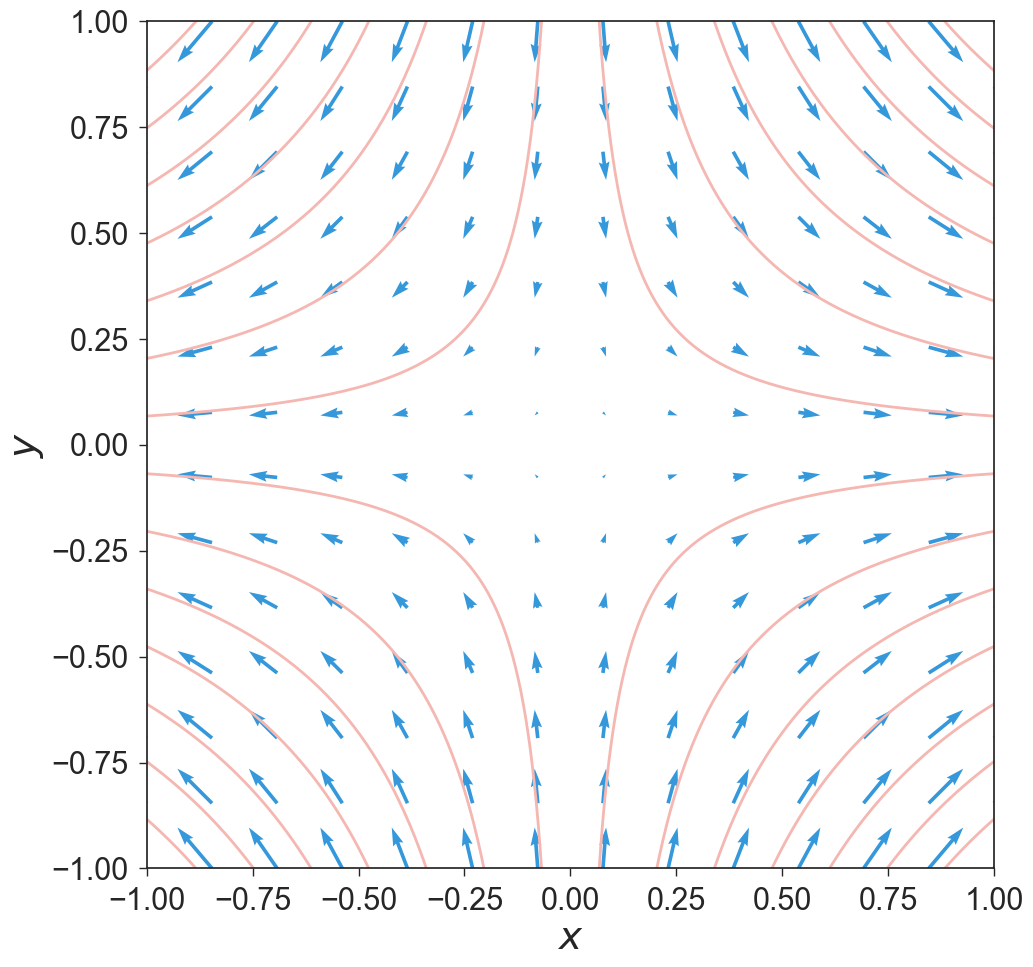
\includegraphics[height=0.85\textwidth]{Saddle-PhasePlot-SIAM.png}
		\end{minipage}
		\begin{minipage}{0.45\textwidth}
			\centering
			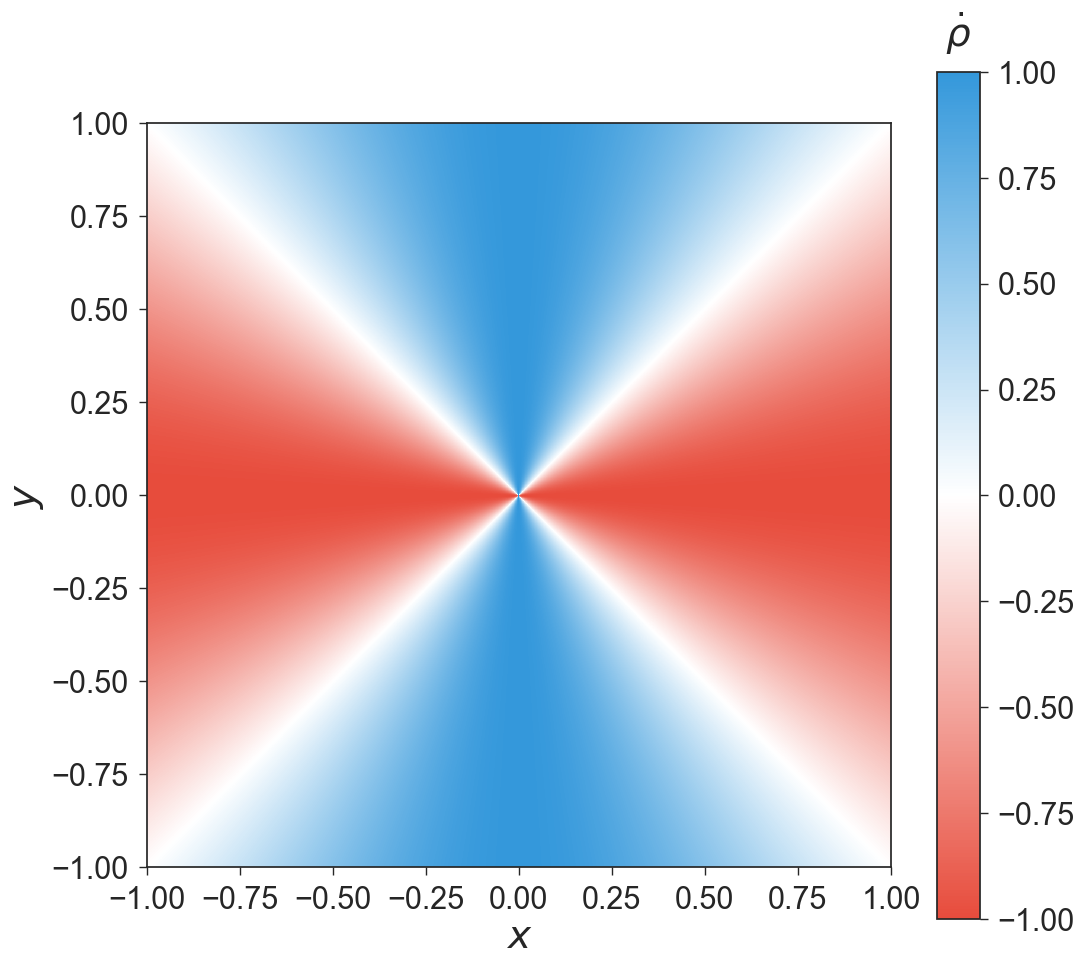
\includegraphics[height=0.85\textwidth]{Saddle-RepRate-SIAM.png}
		\end{minipage}
		\caption{The trajectory-normal repulsion rate field (left) and trajectory-normal repulsion ratio rate field (right) for Example 1.}
		\label{fig: saddle}
	\end{figure*}
	
	\subsection{Slow-fast systems}
	The trajectory-normal repulsion rate proves quite effective at finding slow manifolds of slow-fast systems. The slow manifold is instantaneously attracting or repelling in the fast direction. 
	
	\noindent \textbf{Example 2: Overdamped bead on a rotating hoop.} This example comes from Strogatz \cite{strogatz_nonlinear_2014} Section 3.5, providing a nice example of a slow-fast system. Trajectories collapse quickly to the curve $\Omega = f(\phi)$, where $f(\phi) = \sin\phi (\gamma \cos\phi - 1)$, and then ooze along it toward one of several fixed points.
	
	\begin{equation}
	\begin{aligned}
	\dot{\phi} & = \Omega \\
	\dot{\Omega } & = \frac{1}{\varepsilon}\left(\sin\phi(\gamma\cos\phi - 1) - \Omega\right)
	\end{aligned}
	\label{eq: ex3 rotHoop}
	\end{equation}
	
	Figure \ref{fig:rotHoopA} shows that the repulsion rate is quite effective at capturing the slow manifold. The red curve represents the attracting slow manifold onto which all trajectories converge, as highlighted in Strogatz's textbook example. The repulsion rate disappears near the equilibria of the system which are found each time the curve crosses the horizontal axis. As the repulsion rate is calculated with normal vectors which are normalized by the magnitude of velocity, it is undefined at precisely the equilibria of the system.
	
	\begin{figure*}[t]
		\begin{minipage}{0.45\textwidth}
			\centering
			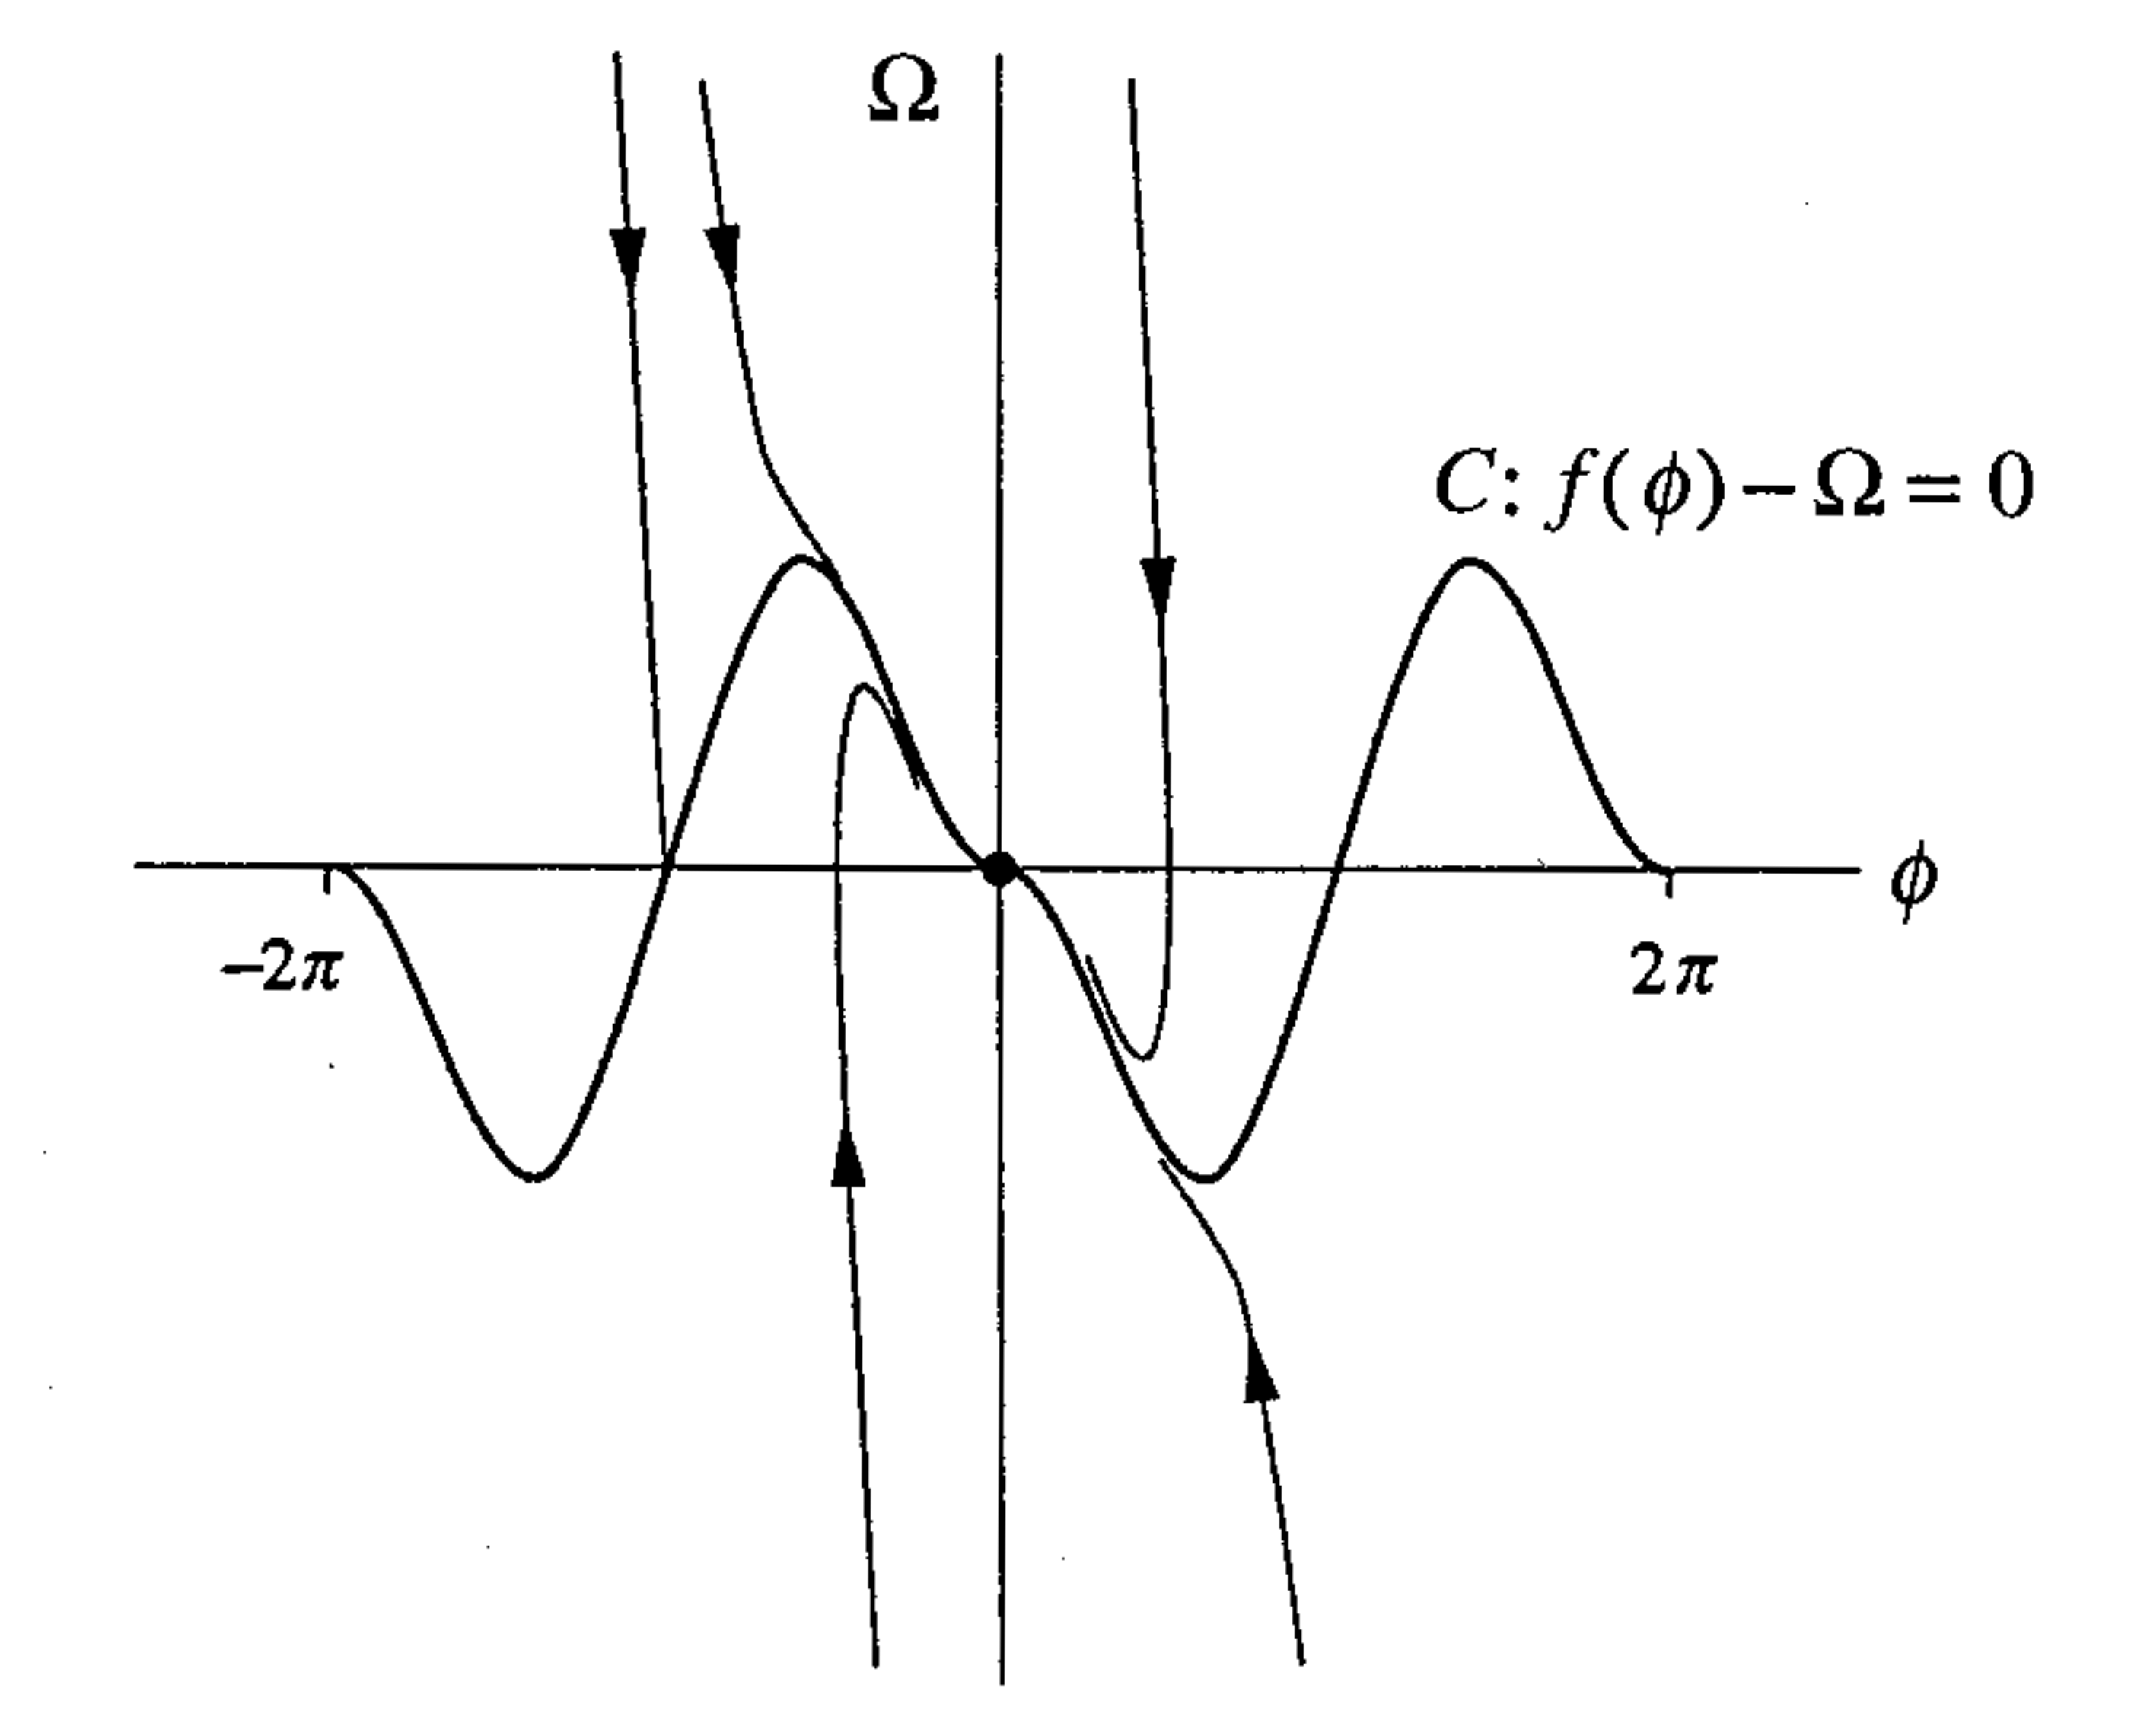
\includegraphics[height=0.7\textwidth]{Strogatz-high-damping-bead-on-hoop.png}
		\end{minipage}	
		\begin{minipage}{0.45\textwidth}
			\centering
			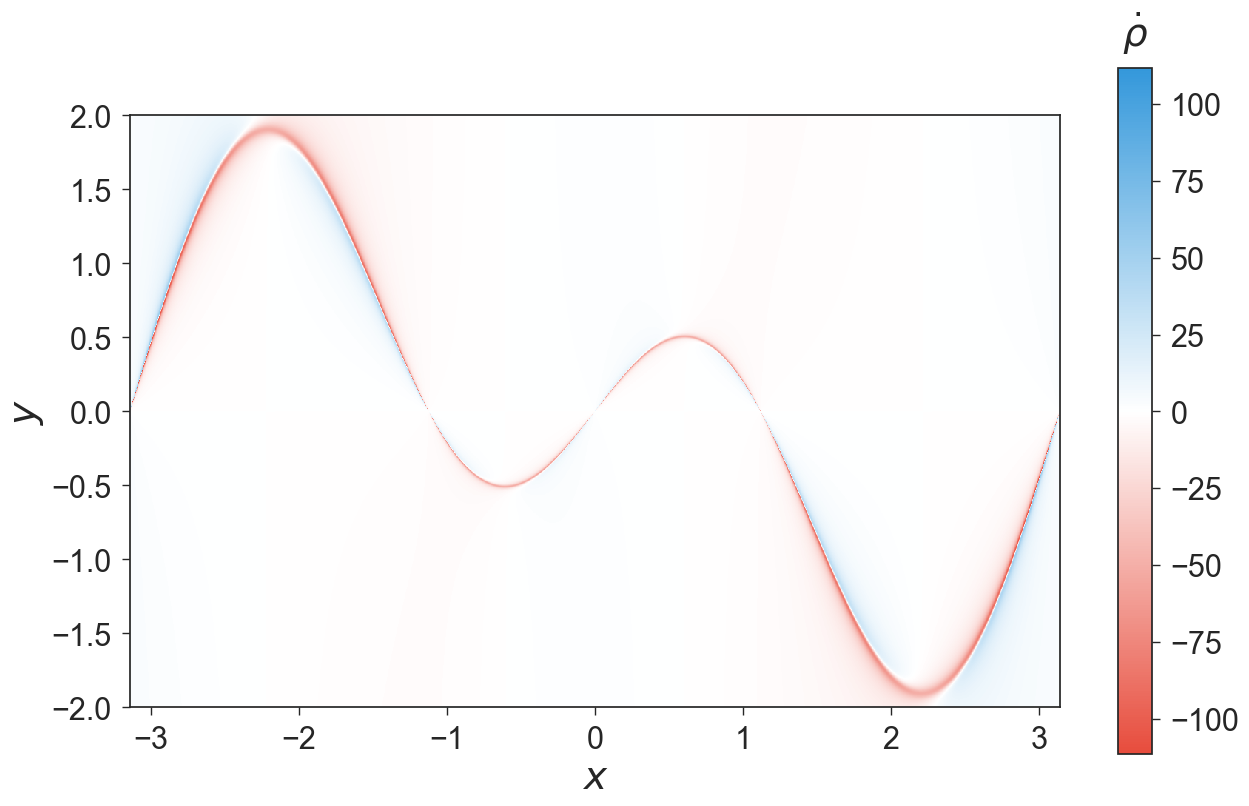
\includegraphics[height=0.7\textwidth]{rotHoop-RepRate-SIAM.png}
		\end{minipage}
		\caption{\label{fig:rotHoopA} (Left) Figure 3.5.8 of \cite{strogatz_nonlinear_2014} showing the schematic of the slow manifold in the overdamped bead in a rotating hoop.	
			(Right) Using the trajectory-normal repulsion rate $\dot \rho$ to find the slow manifold for (\ref{eq: ex3 rotHoop}) in Example 2, using $\varepsilon = 0.01$ and $\gamma = 2.3$.}
	\end{figure*}
	
	\noindent \textbf{Example 3: Verhulst \cite{verhulst2007singular}.} This example system resembles a transcritical bifurcation with a continuously increasing parameter. When $x < 0$, the $x$-axis is an attracting slow manifold and $y=x$ is a repelling slow manifold. When $x > 0$, the $x$-axis is repelling and $y=x$ is attracting.
	\begin{equation}
	\begin{aligned}
	\dot{x} &= 1 \\
	\dot{y} &= \frac{1}{\varepsilon} \left(xy-y^2\right)
	\end{aligned}
	\end{equation}
	
	We can calculate $\dot{\rho}$ for this system using the method described above. We begin by calculating $\mathbf{n}$ and $\mathbf{S}$.
	\begin{equation*}
	\mathbf{n} = \frac{1}{\sqrt{1+\frac{1}{\varepsilon^2}\left(xy-y^2\right)^2}} \left[\begin{array}{c}
	-\frac{1}{\varepsilon} \left(xy-y^2\right) \\
	1
	\end{array}\right]
	\end{equation*}
	
	\begin{equation*}
	\mathbf{S} = \left[\begin{array}{cc}
	0 & \frac{y}{2\varepsilon} \\
	\frac{y}{2\varepsilon} & \frac{1}{\varepsilon}\left(x-2y\right)
	\end{array}\right]
	\end{equation*}
	
	We can find the trajectory-normal repulsion rate using the relation $\dot{\rho}=\mathbf{n}^*\mathbf{S}\mathbf{n}$
	\begin{equation*}
	\dot{\rho} = \frac{y^2\left(y-x\right)+\varepsilon\left(x-y\right)-\varepsilon y}{\varepsilon^2 + \left(x-y\right)^2y^2}
	\end{equation*}
	
	Along $y=0$, we find that the repulsion rate is given by $\dot{\rho} = x/\varepsilon$. Therefore, when $x < 0$, $\dot{\rho}<0$ and this manifold is attracting and when $x > 0$, $\dot{\rho}>0$ and this manifold is repelling. Similarly, along $y=x$, $\dot{\rho} = -y/\varepsilon = -x/\varepsilon$, and the slow manifold is repelling left in the bottom left and attracting in the upper right. The repulsion rate and repulsion ratio rate fields are shown in Figure \ref{fig: verhulst}.
	
	In dynamical systems, it is common to think about stable and unstable invariant manifolds in relation to a fixed point in a flow. However, as in this example, there may be attracting or repelling manifolds without the flow containing any equilibria. The calculation of CECSs allows for detection of structures without any notion of fixed points.
	
	\begin{figure*}[t!]
		\centering
		\begin{minipage}{0.45\textwidth}
			\centering
			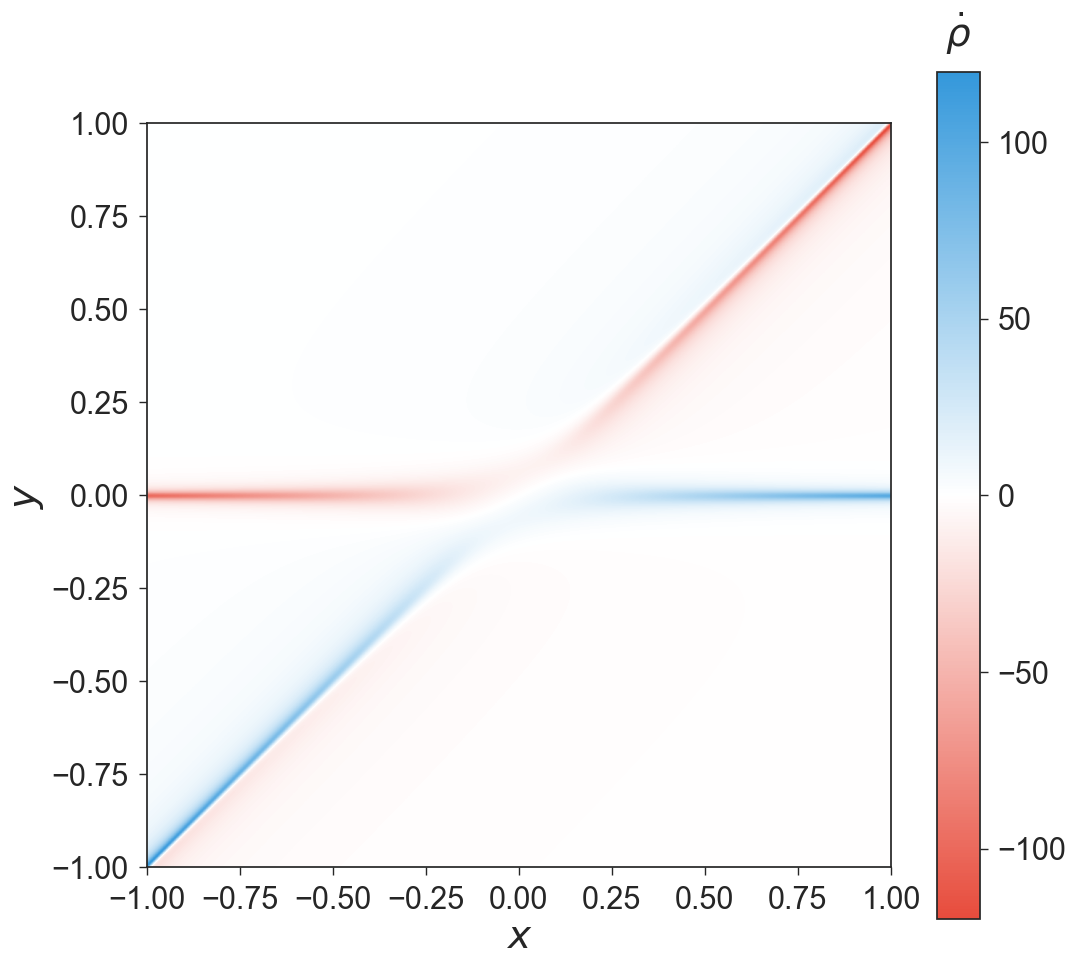
\includegraphics[width=\textwidth]{Verhulst-RepRate-SIAM.png}
		\end{minipage}
		\begin{minipage}{0.45\textwidth}
			\centering
			\includegraphics[width=\textwidth]{Verhulst_RepRatio-SIAM.png}
		\end{minipage}
		\caption{The trajectory-normal repulsion rate field (left) and trajectory-normal repulsion ratio rate field (right) for Example 3 with $\varepsilon=0.001$.}
		\label{fig: verhulst}
	\end{figure*}
	
	\section{Discussion}
	In this work, we develop the notion of hyperbolic constrained Eulerian coherent structures, which represent the instantaneously most attracting or repelling invariant manifolds in a flow. These CECSs can be found through the trajectory-free calculation of the trajectory-normal repulsion rate, which is the leading-order behavior of the trajectory-normal repulsion factor. This calculation provides a fast and effective tool for searching dynamical systems for attracting or repelling structures.
	
	There are many next steps for the testing and application of these methods. The two most pressing are extensions to higher dimensions and to non-autonomous systems. In three-dimensions, the tangent space to an individual trajectory remains one-dimensional, allowing for infinitely many unit vectors normal to the velocity direction. However, effectively developing the tools to use this technique in 3-dimensions could lead to very fast computation of two-dimensional invariant manifolds. For non-autonomous systems, it will be interesting to see the relationship between the instantaneous CECSs and Lagrangian coherent structures in the system.
	
	Constrained Eulerian coherent structures are computationally efficient and physically intuitive. Our hope is that these structures and the trajectory-normal repulsion rate become useful tools for colleagues to investigate many applications, particularly those with attracting slow manifolds. The python package ManID for manifold identification, developed for this paper, may be found on GitHub at \href{https://github.com/gknave/manid}{https://github.com/gknave/manid}.
	
	%	\bibliographystyle{shane-unsrt}
	\bibliographystyle{elsarticle-num}
	%	\bibliographystyle{humannat}
	\bibliography{repulsion-rate-nave-ross}
	
	\appendix
	
	\section{Derivation of Equation (\ref{eq: Repulsion Rate})} \label{ap: normal derivation}
	Starting with (\ref{eq: local Rho}), we find that the trajectory-normal repulsion factor, \(\rho_T\) can be written, to leading order in $T$, as,
	\begin{equation}
	\begin{aligned}
	\rho_T &= 1+ \left(\text{tr}(\mathbf{S})-\frac{\mathbf{v}^*\mathbf{S}\mathbf{v}}{\left|\mathbf{v}\right|^2}\right)T \\
	&= 1+ \frac{1}{\left|\mathbf{v}\right|^2}(\text{tr}(\mathbf{S})\left|\mathbf{v}\right|^2-\mathbf{v}^*\mathbf{S}\mathbf{v})T  \\
	&= 1+ \frac{\mathbf{v}^*(\text{tr}(\mathbf{S})\mathbf{I} - \mathbf{S})\mathbf{v}}{\left|\mathbf{v}\right|^2}T
	\end{aligned}
	\end{equation}
	
	For a 2-tensor, \(\mathbf{A}\), we can write the relation \(\text{tr}(\mathbf{A})\mathbf{I}-\mathbf{A}\) in index notation as \(A_{ii}\delta_{jk} - A_{jk}\).
	\begin{equation}
	\begin{aligned}
	\text{tr}(\mathbf{A})\mathbf{I}-\mathbf{A} &= A_{ii}\delta_{jk} - A_{jk} \\
	&= A_{il}\delta_{li}\delta_{jk} - A_{il}\delta_{lk}\delta_{ji} \\
	&= A_{il}(\delta_{li}\delta_{jk} - \delta_{lk}\delta_{ji}) \\ 
	&= A_{il}\varepsilon_{lj}\varepsilon_{ik} \\
	&= \mathbf{R}^*\mathbf{A}\mathbf{R}
	\end{aligned}
	\end{equation}
	Where \(\varepsilon_{ij}\) is the two-dimensional Levi-Cevita symbol which, for a 2x2 matrix, is the index representation of the negative of the $90^\circ$ counter-clockwise rotation matrix,  $\varepsilon_{ij} = -\mathbf{R}$. Therefore, we can write \(\rho_T\) for small time $T$ as 
	\begin{equation}
	\begin{aligned}
	\rho_T &= 1+ \frac{\mathbf{v}^*(\mathbf{R}^*\mathbf{S}\mathbf{R})\mathbf{v}}{\left|\mathbf{v}\right|^2}T \\
	& = 1+ \frac{(\mathbf{R}\mathbf{v})^*\mathbf{S}(\mathbf{R}\mathbf{v})}{\left|\mathbf{v}\right|^2}T 
	\end{aligned}
	\end{equation}
	Which can  alternatively be written in terms of the unit normal field, \(\mathbf{n} = \mathbf{R}\mathbf{v}/\left|\mathbf{v}\right|\), as in (\ref{unit_vector_fields}), yielding
	\begin{equation}
	\rho_T 
	= 1+ \langle \mathbf{n},\mathbf{S}\mathbf{n} \rangle T 
	\end{equation}	
	which gives us that the leading order behavior is defined by the instantaneous rate,
	\begin{equation}	
	\dot \rho = \langle \mathbf{n},\mathbf{S}\mathbf{n} \rangle
	\end{equation}
	Note that the rate of length change for an infinitesimal material element vector $\ell$ based at $\mathbf{x}_0$ and advected under the flow is
	\begin{equation}
	\frac{d}{dt} |\ell| = \frac{1}{| \ell |} \langle \ell,\mathbf{S}\ell \rangle
	\end{equation}	
	%\begin{equation}
	%\frac{1}{2} \frac{d}{dt} |\ell^2| = \langle \ell,\mathbf{S}\ell \rangle
	%\end{equation}	
	Thus, the leading order behavior of the trajectory-normal repulsion factor for short time \(T\) can be thought of as the rate  of stretching of unit normal vectors, normal to the invariant manifold passing through $\mathbf{x}_0$.
	This value is locally maximized along the most repulsive (or attractive) manifolds, which provide the most influential core of phase space deformation patterns.
	
\end{document}